\documentclass{article}
\usepackage{tikz}

\begin{document}

\newcommand{\eqncircle}{
	\begin{center}
		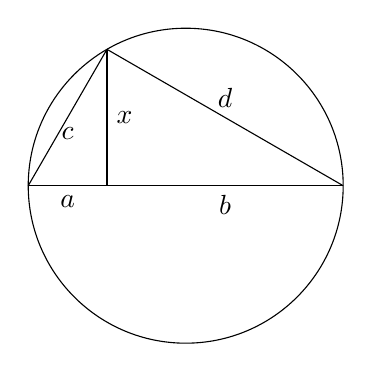
\begin{tikzpicture}
			\draw (2,2) circle (2);
			\draw (0,2) -- node [anchor=north] {$a$} (1,2);
			\draw (1,2) -- node [anchor=north] {$b$} (4,2);
			\draw (1,2) -- node [anchor=west] {$x$} (1,2 + 3^0.5);
			\draw (0,2) -- node [anchor=north] {$c$} (1,2 + 3^0.5);
			\draw (4,2) -- node [anchor=south] {$d$} (1,2 + 3^0.5);
		\end{tikzpicture}
	\end{center}
}

\paragraph{}
Class assigned problem:

\eqncircle{}
\begin{equation}
c^2 + d^2 = (a + b)^2
\end{equation}
\begin{equation}
c^2 = a^2 + x^2
\end{equation}
\begin{equation}
d^2 = b^2 + x^2
\end{equation}


\paragraph{}


\end{document}